\documentclass[../main/main.tex]{subfiles}
\begin{document}
\raggedbottom

% \dominitoc
% \faketableofcontents
% \dominilof
% \fakelistoffigures
% \dominilot
% \fakelistoftables

\chapter{\'Evolution avec le redshift}\label{ch:stretch}
\epigraph{\openquote\textit{We are not to tell nature what she's gotta be. …
She's always got better imagination than we have.}\closequote}{Richard
\textsc{Feynman}}

Comme présenté Chapitre~\ref{ch:sne}, la nature détaillée des SNe~Ia reste
incertaine, et à mesure que les statistiques des relevés augmentent, la question
des incertitudes systématiques astrophysiques se pose, notamment celle de
l'évolution des populations de SNe~Ia. Dans cette perspective, nous avons
discuté Chapitre~\ref{ch:env} des tentatives d'amélioration de notre
connaissance de la physique des SNe~Ia par le biais de l'étude de corrélations
entre leurs propriétés et leur environnement. Nous avons montré l'existence d'un
biais en lien avec la masse globale de la galaxie hôte d'une SN, et mis en
évidence l'exitence de sous-populations basées sur l'âge qui pourraient être
plus pertinentes en tant que traceur de la différence des propriétés observées
dans les SNe.

Notre thèse s'appuie sur cette hypothèse et le lien établi
par~\cite{rigault2020} entre l'étirement des SNe et leur âge. Dans ce chapitre,
nous étudions la dépendance au redshift de l'étirement de courbe de lumière issu
d'un ajustement par \texttt{SALT2.4} de SNe~Ia, qui est une propriété purement
intrinsèque des SNe, afin de sonder sa dérive potentielle avec le redshift. Nous
modélisons différentes dépendances Section~\ref{sec:xmod} et donnons les
résultats de notre analyse Section~\ref{sec:xres}~: nous y verrons que la dérive
astrophysique des propriétés des SNe~Ia est fortement favorisée et que les
modèles de distribution sous-jacente d'étirements constants avec le redshift
sont exclus comme étant de bonnes représentations des données par rapport à
notre modèle de référence.

\vfill
\minitoc
\vfill

\clearpage

\thispagestyle{plain}
\vspace*{\fill}
\minilof
\vspace*{\fill}
\minilot
\vspace*{\fill}

\newpage

\section{Modélisation de l'étirement}\label{sec:xmod}

Pour modéliser l'évolution de la distribution complète de l'étirement des SNe en
fonction du redshift, nous devons modéliser la distribution de l'étirement des
SNe pour chaque sous-échantillon d'âge, étant donné notre modèle susmentionné de
l'évolution de la fraction des SNe~Ia jeunes et vieilles avec le temps cosmique.
\cite{rigault2020} ont présenté la relation entre l'étirement des SN et la
mesure du LsSFR, un traceur de l'âge des progéniteurs, en utilisant
l'échantillon SNfactory (voir Section~\ref{sec:snf}). Cette relation est
illustrée dans la Fig.~\ref{fig:stretchlssfr} pour les SNe de SNfactory
utilisées dans l'analyse actuelle. Étant donné la structure du nuage de points
étirement-LsSFR, notre modèle de la distribution sous-jacente de l'étirement des
SN~Ia est défini comme suit~:
\begin{itemize}
    \item la distribution de l'étirement de la population la plus jeune
        ($\log(\mathrm{LsSFR})\geq-10,82$) est modélisée comme une distribution
        normale unique $\mathcal{N}(\mu_1, \sigma_1{}^2)$~;
    \item et la distribution de l'étirement de la population la plus âgée
        ($\log(\mathrm{LsSFR})<-10,82$) est modélisée comme un mélange gaussien
        bimodal $a\times \mathcal{N} (\mu_1, \sigma_1{}^2) + (1-a)\times
        \mathcal{N}(\mu_2, \sigma_2{}^2)$, où un mode est le même que pour la
        population jeune, $a$ représentant l'effet relatif des deux modes.
\end{itemize}

\begin{figure}
    \centering
    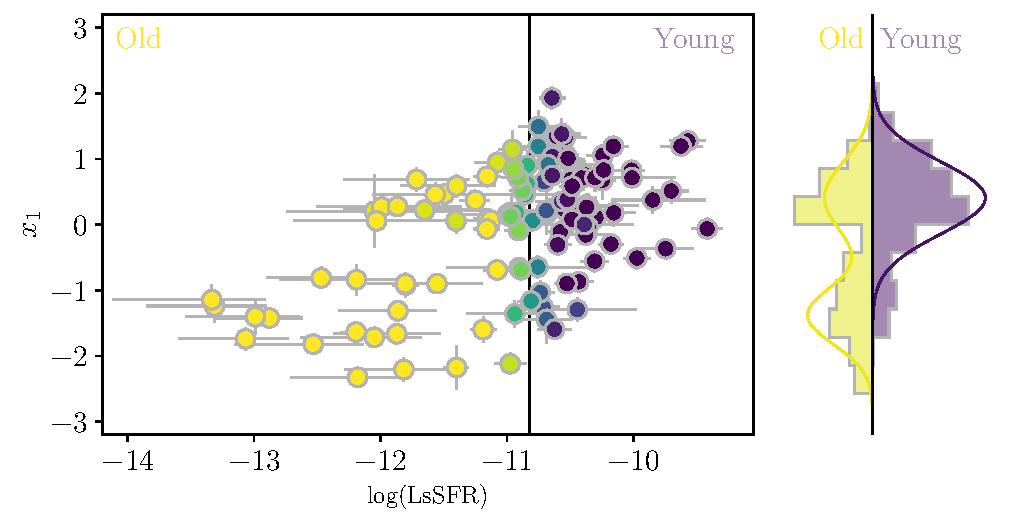
\includegraphics[width=\linewidth]{model_base_hist.pdf}
    \caption[Étirement en fonction du LsSFR des SNe~Ia de SNfactory et modèles
    d'étirement de base ajustés]{\textit{Principal}: étirement de courbe de
        lumière ($x_1$) issu d'un ajustement par \textsc{\texttt{SALT2.4}} en
        fonction du LsSFR pour les SNe de SNfactory. La couleur correspond à la
        probabilité $p_y$ que la SN~Ia soit jeune, c'est-à-dire qu'elle ait
        $\log\mathrm{LsSFR} \geq -10.82$ \citep[voir][]{rigault2020}. \textit{À
        droite}: histogramme pondéré par $p_y$ des étirements des SNe, ainsi que
        le modèle de base ajusté~; les contributions de la population jeune
    et âgée sont indiquées en violet et en jaune, respectivement.}
    \label{fig:stretchlssfr}
\end{figure}

La fonction de distribution de probabilité (pdf) de l'étirement d'une SN donnée
sera alors la combinaison linéaire des distributions d'étirement de ces deux
populations, pondérées par sa probabilité $y^i$ d'être jeune. Pour en décrire
l'évolution avec le redshift, nous utilisons une association statistique donnée
par la probabilité qu'une SN soit jeune en fonction de son redshift, décrite par
la fraction de jeunes SNe~Ia et donnée par $\delta(z)$ (voir
Équation~\ref{eq:deltaz}). Notre modèle de dérive avec le redshift de la moyenne
de la distribution sous-jacente d'étirement $X_1(z)$ est alors donnée par~:
\begin{align}\label{eq:stretchz}
    X_1(z) = \delta(z)&\times \mathcal{N}(\mu_1,\sigma_1{}^2) + \nonumber \\
    (1-\delta(z))&\times \left[ a\times\mathcal{N}(\mu_1,\sigma_1{}^2) +
    (1-a)\times\mathcal{N}(\mu_2,\sigma_2{}^2) \right]
\end{align}
Ceci constitue notre modèle de dérive de base.

\subsection{Paramétrisations}\label{ssec:pmod}

Compte tenu de la probabilité $y^i$ qu'une SN donnée soit jeune et supposant
notre modèle de base (voir Section~\ref{sec:xmod}), la probabilité de
mesurer un étirement \texttt{SALT2.4} $x_1^i$ avec une erreur $\d x_1^i$ est
donné par~:
\begin{align}\label{eq:likelihoodsnf}
    \prob{x^i_1}{\overrightarrow{\theta}; \mathrm{d}x^i_1, y^i} =
    y^i & \times
    \mathcal{N}\left(x^i_1 \mid \mu_1, \sigma_1{}^2+\mathrm{d}x^i_1{}^2\right) +
    \nonumber\\
    (1-y^i) &\times \bigg[
    a \times \mathcal{N}\left(x^i_1 \mid \mu_1,
    \sigma_1{}^2+\mathrm{d}x^i_1{}^2\right) +
    \nonumber\\
    & (1-a) \times \mathcal{N}\left(x^i_1 \mid \mu_2,
    \sigma_2{}^{2}+\mathrm{d}x^i_1{}^2\right) \bigg]
\end{align}

L'estimation du maximum de vraisemblance des cinq paramètres libres
$\overrightarrow{\theta}\equiv({\mu_1, \mu_2, \sigma_1, \sigma_2,a})$ du modèle
s'obtient en minimisant l'équation suivante~:

\begin{equation}\label{eq:likelihood}
    -2\ln(L) = -2 \sum_i \ln \prob{x_1^i}{\overrightarrow{\theta};
    \mathrm{d}x_1^i, y^i}
\end{equation}
Selon que nous pouvons estimer $y^i$ directement à partir des mesures de LsSFR
ou non, il y a deux façons de procéder. Nous les décrivons ci-dessous.

\subsubsection*{Avec LsSFR}\label{sssec:lssfr}

Pour l'échantillon SNfactory, nous pouvons facilement fixer $y^i = p_y^i$, la
probabilité d'avoir $\log(\mathrm{LsSFR}) \geq -10,82$ (voir
Figure~\ref{fig:stretchlssfr}) afin de minimiser l'Équation~\ref{eq:likelihood}
par rapport à $\overrightarrow{\theta}$. Les résultats de l'ajustement de ce
modèle avec les SNe~Ia de SNf sont présentés dans le
Tableau~\ref{tab:modelresults} et illustrés Figure~\ref{fig:evol_all}.

\begin{table*}
    \centering
    \caption[Valeurs des paramètres du modèle d'étirement de base selon
    l'échantillon]{Valeurs des paramètres issus des meilleurs ajustements du
        modèle de distribution de l'étirement de base lorsqu'il est
        appliqué à l'ensemble de données de SNfactory seulement (114 SNe~Ia), à
        l'échantillon fiduciel (569 SNe~Ia) ou à l'échantillon conservatif
    (422).}
    \label{tab:modelresults}
    \begin{tabular}{lccccc}
        \toprule
        Échantillon & $\mu_1$             & $\sigma_1$
                    & $\mu_2$             & $\sigma_2$
                    & $a$ \\
        \midrule
        SNfactory   & $ 0.41 \pm 0.05$    & $0.55 \pm 0.04$
                    & $-1.38 \pm 0.07$    & $0.44 \pm 0.06$
                    & $ 0.48 \pm 0.06$ \\
        Fiduciel    & $ 0.37 \pm 0.04$    & $0.61 \pm 0.03$
                    & $-1.22 \pm 0.11$    & $0.56 \pm 0.07$
                    & $ 0.51 \pm 0.07$ \\
        Conservatif & $ 0.38 \pm 0.04$    & $0.60 \pm 0.03$
                    & $-1.26 \pm 0.09$    & $0.53 \pm 0.06$
                    & $ 0.47 \pm 0.06$ \\
        \bottomrule
    \end{tabular}
\end{table*}

\subsubsection*{Sans LsSFR}\label{sssec:z}

Lorsque les mesures directes de LsSFR font défaut (c'est-à-dire en absence de
$p_y^i$), nous pouvons étendre cette analyse aux échantillons autres que
SNfactory en utilisant l'évolution avec le redshift de la fraction $\delta(z)$
des jeunes SNe~Ia (Équation~\ref{eq:deltaz}) comme un indicateur alternatif de
la probabilité qu'une SN soit jeune correspondant à son
prior\footnote{C'est-à-dire la probabilité qu'une SN soit jeune étant donné son
redshift.}. Cela implique toujours la minimisation de
l'Équation~\ref{eq:likelihood} par rapport aux paramètres 
$\overrightarrow{\theta}\equiv(\mu_1, \mu_2, \sigma_1, \sigma_2, a)$ de la
distribution d'étirement $X_1$ (Équation~\ref{eq:likelihoodsnf}) mais en
supposant cette fois que $y^i = \delta(z^i)$ pour une SN $i$ donnée.

Pour le reste de cette analyse, nous avons ainsi ajusté
l'Équation~\ref{eq:likelihood} en utilisant $p_y^i$ la probabilité que la SN $i$
soit jeune lorsqu'elle est disponible (c'est-à-dire pour les données de
SNfactory) et $\delta(z^i)$, la fraction attendue de jeunes SNe~Ia au redshift
$z^i$ de la SN sinon.\bigbreak

Les résultats de l'ajustement de ce modèle à l'ensemble des 569 (respectivement
422) SNe~Ia de l'échantillon fiduciel (conservatif) sont présentés dans le
Tableau~\ref{tab:modelresults}, et l'évolution prédite de l'étirement avec le
redshift ($x_1$ attendu compte tenu de la distribution de
l'équation~\ref{eq:stretchz}) est illustrée sous la forme d'une bande bleue dans
la Figure~\ref{fig:evol_all}, qui tient compte des erreurs des paramètres et de
leurs covariances. Cette figure montre que l'étirement moyen mesuré des SNe~Ia
par intervalle de redshift (contenant tous le même nombre de données) suit de
près notre modélisation de la dérive avec le redshift. C'est en effet ce que
nous attendons si les environnements vieux favorisent les faibles étirements de SN
\citep[voir par exemple][]{howell2007} et si la fraction de vieilles SNe~Ia
diminue en fonction du redshift. Nous discutons quantitativement de ces
résultats Section~\ref{sec:xres}.

\begin{figure}
%    \centering
    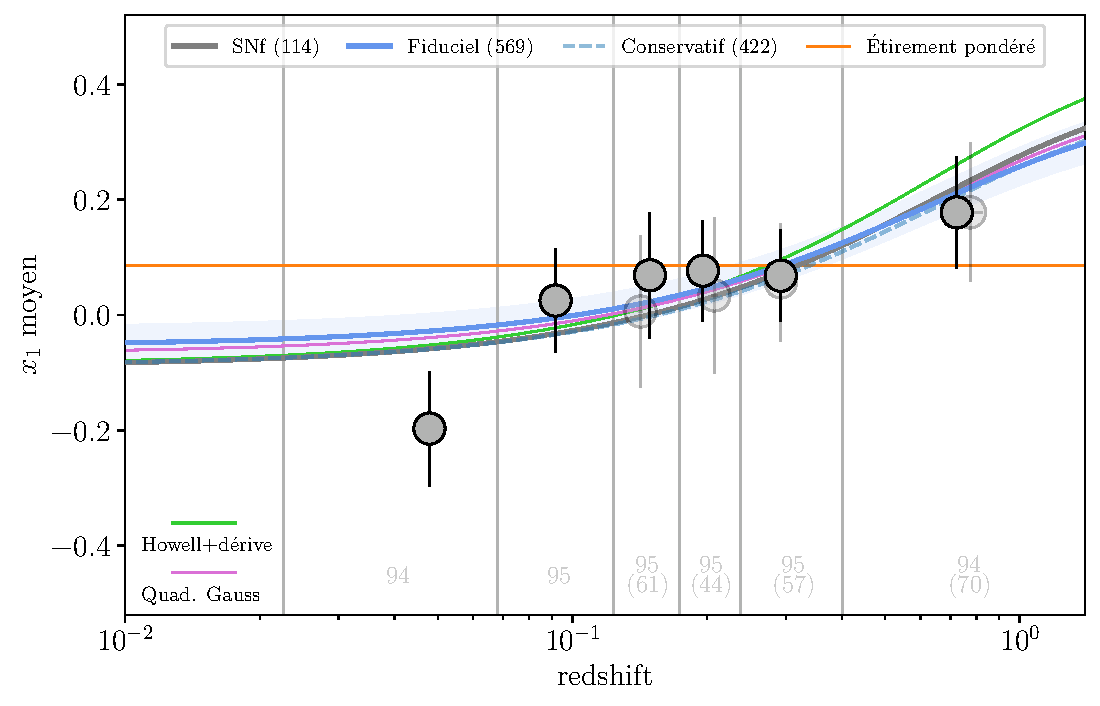
\includegraphics[width=\linewidth]{stretchevol_all-oth_vs_snf-weighted.pdf}
    \caption[Évolution de l'étirement moyen des SNe~Ia en fonction du redshift
    issu de la prédiction de notre modèle de base selon l'échantillon
    utilisé]{Évolution de l'étirement moyen ($x_1$) des SNe~Ia issus d'un
        ajustement \texttt{SALT2.4} en fonction du redshift pour notre modèle de
        base. Les marqueurs montrent la moyenne pondérée de l'étirement mesurée
        dans des intervalles de redshift de tailles d'échantillon égales,
        indiquées en gris clair en bas de chaque intervalle. Les marqueurs
        opaques et transparents sont utilisés lorsque les échantillons fiduciel
        ou conservatif sont considérés, respectivement. La ligne horizontale
        orange représente l'étirement pondéré des données. Les meilleurs
        ajustements de notre modèle de dérive de base sont présentés en bleu,
        bleu pointillé et gris lorsqu'ils sont ajustés sur l'échantillon
        fiduciel, conservatif ou l'ensemble de données SNfactory uniquement,
        respectivement~; ils sont tous compatibles entre eux et avec les
        données. La bande bleu clair illustre l'amplitude de l'erreur
        (covariance comprise) du modèle le mieux ajusté lorsque nous considérons
        l'ensemble de données fiduciel. Les lignes verte et violette
        représentent les meilleurs ajustements d'autres modèles dérivants, voir
    Sections~\ref{ssec:modimpl},~\ref{ssec:testsupp}.}
    \label{fig:evol_all}
\end{figure}

\subsection{Implémentation}\label{ssec:modimpl}

Dans la Section~\ref{ssec:pmod}, nous avons modélisé la distribution
sous-jacente de l'étirement des SNe~Ia en suivant~\cite{rigault2020},
c'est-à-dire avec une unique Gaussienne pour les jeunes SNe et un mélange de
deux Gaussiennes pour la population des vieilles SNe~Ia, la première étant la
même que pour la jeune population et la seconde étant spécifique aux SNe à
déclin rapide, qui semblent n'exister que dans les environnements localement
vieux. C'est ce que nous appelons notre modèle de base. Cependant, pour
tester différents choix de modélisation, nous avons mis en œuvre une suite de
paramétrisations alternatives que nous avons également ajustées aux données en
suivant la procédure décrite dans la Section~\ref{ssec:pmod}.

\cite{howell2007} ont utilisé un modèle unimodal plus simple par catégorie
d'âge, en supposant une distribution normale unique pour chacune des populations
jeune et âgée. Nous avons donc considéré un modèle «~Howell+dérive~», comportant
une seule Gaussienne par groupe d'âge et intégrant la dérive avec $\delta(z)$ de
l'équation~\ref{eq:deltaz}. L'évolution moyenne de l'étirement avec le redshift
de ce modèle est tracée en vert Figure~\ref{fig:evol_all}.

Alternativement, comme nous cherchons à vérifier l'existence d'une évolution
avec le redshift, nous avons également testé des modèles constants en limitant
les modèles de base et de \textsc{Howell} à utiliser une fraction de jeunes
SNe~Ia $\delta(z) \equiv f$ indépendante du redshift~; ces modèles sont appelés
ci-après «~base+constant~» et «~Howell+constant~».

Nous avons également considéré un autre modèle intrinsèquement non-dérivant, la
forme fonctionnelle développée pour la méthode \textit{BEAMS with Bias
Correction}~\citep[BBC,][]{scolnic2016, kessler2017}, utilisée dans les analyses
cosmologiques utilisant les SNe~Ia les plus récentes~\citep[par
exemple][]{scolnic2018, abbott2019, riess2016, riess2019} pour tenir compte des
biais de \textsc{Malmquist}. Le formalisme de BBC suppose des distributions
d'étirement Gaussiennes asymétriques basées sur la forme de chaque échantillon
(et donc intrinsèquement sans dérive)~: $\mathcal{N}\left(\mu, \sigma_-{}^2\;
\text{si} \;x_1<\mu,\; \text{sinon} \;\sigma_+{}^2\right)$. L'idée derrière
cette approche par échantillon est double~\citep{scolnic2016, scolnic2018}~:
\begin{enumerate}
    \item les biais de \textsc{Malmquist} sont déterminés par les propriétés des
        relevés~;
    \item comme les relevés actuels couvrent des plages de redshift limitées,
        une approche par échantillon couvre certaines informations potentielles
        sur l'évolution avec le redshift.
\end{enumerate}
Une discussion plus détaillée sur BBC se trouve Section~\ref{ssec:disc}. Enfin,
par souci d'exhaustivité, nous avons également considéré des modèles Gaussiens
purs et asymétriques indépendants du redshift.

\section{Résultats}\label{sec:xres}

Nous exposons maintenant les résultats quantitatifs de cette étude
Section~\ref{ssec:xcomp}, et proposons une discussion de ceux-ci
Section~\ref{ssec:disc}.

\subsection{Comparaison aux données}\label{ssec:xcomp}
Nous avons ajusté chacun des modèles décrits ci-dessus sur les échantillons
fiduciel et conservatif (voir Chapitre~\ref{ch:sample}). Les résultats sont
rassemblés dans le Tableau~\ref{tab:comp} et sont illustrés
Figure~\ref{fig:mod_comp}.

\begin{table}[ht]
    \centerfloat
    \begin{threeparttable}
    \caption[Comparaison de la capacité relative de chaque modèle à décrire les
    données par rapport au modèle de base]{Comparaison de la capacité relative
    de chaque modèle à décrire les données.} \label{tab:comp}
        % \makebox[\linewidth]{%
        \begin{tabular}{lcccccccc}
            \toprule
            & & & \multicolumn{3}{c}{Échantillon fiduciel (569 SNe)}
                & \multicolumn{3}{c}{Échantillon conservatif (422 SNe)} \\
            \cmidrule(lr){4-6} \cmidrule(lr){7-9}
            Nom & dérive & $k$ &
            $-2\ln(L)$ & AIC & $\Delta$AIC & $-2\ln(L)$ & AIC & $\Delta$AIC\\
            \midrule
            Base & $\delta(z)$ & 5
            & 1456,7 & 1466,7 & -- 
            & 1079,5 & 1089,5 & -- \\
            Howell+dérive & $\delta(z)$ & 4
            & 1463,3 & 1471,3 & $-4,6$
            & 1088,2 & 1096,2 & $-6,7$ 
            \\
            Asymétrique & -- & 3
            & 1485,2 & 1491,2 & $-24,5$
            & 1101,3 & 1107,3 & $-17,8$ 
            \\
            Howell+constant & $f$ & 5
            & 1484,2 & 1494,2 & $-27,5$
            & 1101,2 & 1111,2 & $-21,7$ 
            \\
            Base+constant & $f$ & 6
            & 1484,2 & 1496,2 & $-29,5$
            & 1101,2 & 1113,2 & $-23,7$ 
            \\
            Asym.\ par échant. & Par échant. & 3$\times$5
            & 1468,2 & 1498,2  & $-31,5$
            & 1083,6 & 1113,6  & $-24,1$ 
            \\
            Gaussienne & -- & 2
            & 1521,8 & 1525,8 & $-59,1$
            & 1142,6 & 1146,6 & $-57,1$ 
            \\
            \bottomrule
        \end{tabular}%}
        \begin{tablenotes}[flushleft]
        \item\small \textbf{\hspace{-3.2pt}Notes.} Pour chaque modèle considéré,
            nous indiquons si le modèle dérive ou non, son nombre de paramètres
            libres $k$, et pour les échantillons fiduciel et conservatif,
            $-2\ln(L)$ (voir Équation~\ref{eq:likelihood}), l'AIC et la
            différence d'AIC ($\Delta$AIC) entre ce modèle et le modèle de base,
            choisi comme référence car présentant l'AIC le plus faible.
        \end{tablenotes}
    \end{threeparttable}
\end{table}

\begin{figure}[ht]
%    \centering
    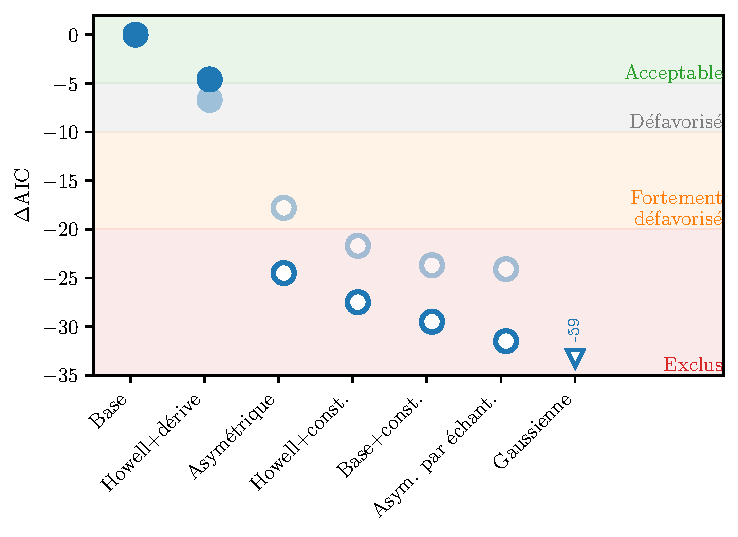
\includegraphics[width=\linewidth]{mod_comp-fr.pdf}
    \caption[$\Delta$AIC entre le modèle de base et les autres
    modèles]{$\Delta$AIC entre le modèle de référence et les autres
        modèles (voir Tableau~\ref{tab:comp}). Les marqueurs bleus pleins et
        ouverts correspondent aux modèles avec et sans dérive du redshift,
        respectivement. Les marqueurs transparents montrent les résultats
        lorsque l'analyse est effectuée sur l'échantillon conservatif plutôt que
        sur l'échantillon fiduciel. Les bandes de couleur illustrent la validité
        des modèles, d'acceptable ($\Delta$AIC > -5) à exclu ($\Delta$AIC <
        -20), voir le corps de texte. En suivant ces valeurs d'AIC, tous les
        modèles sans dérive (marqueurs ouverts) sont exclus car il représentent
    moins bien les données que le modèle de référence, avec dérive.}
    \label{fig:mod_comp}
\end{figure}

Parce que les divers modèles présentent différents degrés de liberté, nous avons
utilisé le critère d'information d'\textsc{Akaike}~\citep[AIC, voir par
exemple][]{burnham2004} pour comparer leur capacité à décrire correctement les
observations. Cet estimateur pénalise l'ajout de degrés de liberté
supplémentaire afin d'éviter un ajustement excessif des données. Il est défini
comme suit~:
\begin{equation}\label{eq:aic}
    \mathrm{AIC} = -2\ln(L) + 2k,
\end{equation}
où $-2\ln(L)$ est obtenu en minimisant l'Équation~\ref{eq:likelihood}, et $k$
est le nombre de paramètres libres à ajuster. Le modèle de référence est celui
de plus petit AIC~; par rapport à ce modèle, les modèles avec $\Delta$AIC > -5
sont qualifiés d'acceptables, ceux avec $-5 > \Delta\mathrm{AIC} > -20$ ne sont
pas favorisés et ceux avec $\Delta$AIC < -20 sont jugés exclus. Cela correspond
approximativement aux limites de 2, 3 et 5$\sigma$ pour une distribution de
probabilité Gaussienne.

Le meilleur modèle (avec le plus petit AIC) est le modèle dit de base et
constitue donc notre modèle de référence~; ceci est vrai pour les échantillons
fiduciel et conservatif. Le modèle de base a également le plus petit $-2\ln(L)$,
ce qui en fait le modèle le plus probable même si nous ne tenons pas compte de
la question de l'ajustement excessif qui est pris en compte par le formalisme de
l'AIC.

En outre, nous constatons que les distributions d'étirement indépendantes du
redshift sont toutes exclues comme descriptions appropriées des données
relativement au modèle de base. Le meilleur modèle  non-dérivant (le modèle
asymétrique) a une chance très marginale ($p \equiv \exp(\Delta\mathrm{AIC}/2) =
\num{5e-6}$) de décrire les données aussi bien que le modèle de base. Ce
résultat n'est qu'une évaluation quantitative de faits qualitatifs qui sont
clairement visibles sur la Figure~\ref{fig:evol_all}~: l'étirement moyen des SNe
par intervalle de redshift suggère fortement une évolution significative du
redshift plutôt qu'une valeur constante, et cette évolution est bien décrite par
l'Équation~\ref{eq:deltaz}.

De manière surprenante, la modélisation asymétrique Gaussienne par échantillon
utilisée par les implémentations actuelles de la technique BBC
\citep{scolnic2016, kessler2017} présente l'une des valeurs d'AIC les plus
élevées de notre analyse. Bien que son $-2\ln(L)$ soit le plus petit de tous les
modèles indépendants du redshift (mais toujours inférieur de \num{11.5} au
modèle de référence), il est fortement pénalisé car il nécessite 15 paramètres
libres ($\mu_0$, $\sigma_{\pm}$ pour chacun des cinq échantillons de l'analyse).
Par conséquent, il en résulte un $\Delta\mathrm{AIC} < -20$, ce qui pourrait
être interprété comme une probabilité $p = \num{2e-7}$ d'être une aussi bonne
représentation des données que le modèle de référence.

Nous notons que lorsque nous comparons des modèles qui ont été ajustés sur des
sous-échantillons individuels plutôt que globalement, le critère d'information
bayésien ($\mathrm{BIC} = -2\ln(L) + k\ln(n)$, avec $n$ le nombre de points de
données) pourrait être plus adapté que l'AIC car il tient explicitement compte
du fait que chaque sous-échantillon est ajusté séparément~: le BIC du modèle par
échantillon est alors la somme des BIC de chaque échantillon. Nous trouvons
$\Delta\mathrm{BIC} = -48$, ce qui réfute également le modèle Gaussien
asymétrique par échantillon comme étant aussi pertinent que notre modèle de
référence.

Afin de s'assurer que nos résultats ne sont pas influencés par le
sous-échantillon HST incomplètement modélisé, nous avons recalculé le
$\Delta$AIC pour chaque modèle en excluant cet ensemble de données~; cela n'a
pas modifié le $\Delta$AIC de plus de quelques dixièmes. La cohérence de ces
valeurs avec celles du Tableau~\ref{tab:comp} montre que le sous-échantillon HST
n'influence pas nos conclusions.

Nous rapportons dans le Tableau~\ref{tab:bbc} notre détermination de $\mu_0$ et
$\sigma_{\pm}$ pour chaque échantillon lorsqu'un modèle Gaussien asymétrique a
été appliqué, et ajusté sur les échantillons normalement sans effets de
sélection en utilisant nos coupes fiducielles (voir Chapitre~\ref{ch:sample}).
Nos résultats sont en accord étroit avec ceux de~\cite{scolnic2016} pour SNLS et
SDSS et avec les résultats rapportés par~\cite{scolnic2018} pour PS1, qui ont
dérivé ces paramètres de modèle en utilisant le formalisme complet BBC. Ce
dernier utilise de nombreuses simulations pour modéliser les effets de
sélection observationnels \citep[voir les détails par exemple Section~3 de][et
le Chapitre~\ref{ch:snana}]{kessler2017}. L'accord entre notre ajustement des
Gaussiennes asymétriques sur la partie supposée sans effets de sélection des
échantillons et les résultats dérivés en utilisant le formalisme BBC soutient
notre approche pour construire un échantillon avec des effets de sélection
observationnels négligeables. Si nous devions utiliser les valeurs les mieux
ajustées de~\cite{scolnic2016} et de~\cite{scolnic2018} pour les paramètres
asymétriques $\mu_0,\sigma_{\pm}$ pour les échantillons SNLS, SDSS et PS1
respectivement, le $\Delta$AIC entre notre modèle de dérive de référence
et la modélisation BBC irait encore plus loin, passant de -32 à -47. Nous
discutons plus en détail de la conséquence de ce résultat pour la cosmologie
dans la Section~\ref{ssec:disc}.

\begin{table}
    \centering
    \caption[Paramètres de meilleur ajustement pour notre modélisation
    asymétrique par échantillon de la distribution d'étirement
    sous-jacente]{Paramètres de meilleur ajustement pour notre modélisation
    asymétrique par échantillon de la distribution d'étirement sous-jacente.}
    \label{tab:bbc}
    \begin{threeparttable}
        \makebox[\linewidth]{%
        \begin{tabular}{lcccccc}
        \toprule
        Asymétrique   & $\sigma_{-}$    & $\sigma_{+}$    & $\mu_0$ \\
        \midrule
        SNfactory     & 1,34 $\pm$ 0,13 & 0,41 $\pm$ 0,10 & 0,68 $\pm$ 0,15 \\
        SDSS\tnote{1} & 1,31 $\pm$ 0,11 & 0,42 $\pm$ 0,09 & 0,72 $\pm$ 0,13 \\
        PS1\tnote{2}  & 1,01 $\pm$ 0,11 & 0,52 $\pm$ 0,12 & 0,38 $\pm$ 0,16 \\
        SNLS\tnote{3} & 1,41 $\pm$ 0,13 & 0,15 $\pm$ 0,13 & 1,22 $\pm$ 0,15 \\
        HST           & 0,76 $\pm$ 0,36 & 0,79 $\pm$ 0,35 & 0,11 $\pm$ 0,44 \\
        \bottomrule
        \end{tabular}}
        \begin{tablenotes}[flushleft]
            \item\small \textbf{\hspace{-3,2pt}Notes.} Nous comparons ces
                valeurs à celles des études intégrant les mêmes distributions
                asymétriques.
            \item [1]\small $\sigma_{-} = 1,65 \pm 0,08$, $\sigma_{+} = 0,10 \pm
                0,10$, $\mu_0 = 1,14 \pm 0,03$ \citep[Tableau~1,][]{scolnic2016}
            \item [2]\small $\sigma_{-} = 0,96 \pm 0,16$, $\sigma_{+} = 0,51 \pm
                0,14$, $\mu_0 = 0,37 \pm 0,21$ \citep[Tableau~3,][]{scolnic2018}
            \item [3]\small $\sigma_{-} = 1,23 \pm 0,10$, $\sigma_{+} = 0,28 \pm
                0,10$, $\mu_0 = 0,96 \pm 0,14$ \citep[Tableau~1,][]{scolnic2016}
        \end{tablenotes}
    \end{threeparttable}
\end{table}

\subsection{Tests supplémentaires}\label{ssec:testsupp}

Nous avons également effectué des tests permettant au mode d'étirement élevé de
la population âgée de différer de celui de la population jeune, ajoutant ainsi
deux degrés de liberté ($\mu_1^{\rm O}, \sigma_1^{\rm O}$, voir ligne 3
Figure~\ref{fig:mod_all}). L'ajustement correspondant n'est pas
significativement meilleur, avec un $\Delta$AIC de \num{-0.4} du fait de la
pénalisation de cet estimateur. Cela renforce notre hypothèse selon laquelle les
populations jeune et âgée semblent effectivement partager le même mode
sous-jacent d'étirement élevé. De plus, nous pouvons nous demander si un mode de
faible étirement pourrait également exister dans la population jeune (voir la
Figure~\ref{fig:stretchlssfr}). Nous avons testé cette hypothèse en permettant à
cette population d'être aussi bimodale, en rajoutant deux
paramètres ($\mu_2^{\rm Y}, \sigma_2^{\rm Y}$, ligne 4
Figure~\ref{fig:mod_all}). Nous avons constaté que l'amplitude d'un tel mode de
faible étirement est fondamentalement 0 dans cette jeune population, n'apportant
aucune amélioration dans la qualité de l'ajustement (même $-2\ln(L)$ que le
modèle de base), et donc discriminé négativement par la réduction de son AIC
($\Delta$AIC = -2,0).

Finalement, nous avons également implémenté un modèle combinant ces deux
hypothèses, c'est-à-dire avec deux Gaussiennes par catégorie d'âge, chacune de
ces quatre Gaussiennes pouvant différer les unes des autres. Celui-ci présente
alors quatre valeurs moyennes sensiblement différentes, d'amplitudes
non-compatibles avec 0 (voir ligne 1 Figure~\ref{fig:mod_all}). Une telle
liberté dans la paramétrisation permet alors à ce modèle d'être considéré comme
une bien meilleure représentation des données que notre modèle de référence,
avec un $\Delta$AIC = 6,17. Sa version constante avec le redshift reste
cependant complètement défavorisée avec un $\Delta$AIC = -32,07. L'évolution
moyenne de l'étirement avec le redshift de ce modèle est représenté en violet
Figure~\ref{fig:evol_all} sous la légende «~Quad. Gauss~». Bien que sa qualité
d'ajustement soit nettement supérieure à notre modèle de base, il n'a pas été
conservé dans cette analyse étant donné la complexité de sa composition, peu
motivée physiquement, et la grande similitude dans l'évolution moyenne en
résultant. Cette implémentation semblerait principalement représenter une limite
à la définition de l'AIC et à sa capacité à permettre de discriminer deux
modèles censés représenter une réalité physique. L'ensemble des modèles testés
sont présentés Figure~\ref{fig:mod_all}.

% , dans
% laquelle les modèles dérivants sont tracés dans la colonne de gauche et leur
% version constante dans la colonne de droite. Les deux modèles ne se basant pas
% sur des catégories d'âge (la simple Gaussienne et la Gaussienne asymétriques)
% sont représentées dans la dernière ligne côte à côte conjointement à
% l'histogramme des étirements de notre échantillon. Les quantités
% $\Delta(-2\ln(L))$ et $\Delta$AIC par rapport au modèle de référence (ligne 2)
% sont indiqués dans les coins extérieurs de chaque figure. Pour les modèles
% dérivants, on en a tracé dix réalisations selon la valeur du redshift moyen
% considéré, de la valeur la plus basse de notre échantillon ($z = 0,02$) à la
% valeur maximale des données totales (sans coupe en redshift) de SNLS ($z =
% 1,06$) représentés en couleur allant du jaune (bas redshift, plus vieil
% environnement) au violet (haut redshift, environnement jeune) et les
% distributions des populations jeune et vieille constituant le modèle total sont
% en gris pointillé et fin pointillé, respectivement. Les modèles non-dérivants
% sont tracés en vert avec les sous-populations vieille et jeune en jaune et
% violet, respectivement. On y retrouve l'information que tous les modèles
% non-dérivants sont exclus en tant que bonnes représentations des données par
% rapport au modèle de base.

\begin{figure}[p]
    \vspace*{-2.8cm}
    \centerfloat
    \includegraphics[width=1.1\linewidth]{model_all_evol.pdf}
%    \captionsetup{justification=centering}
    \caption[Modèles implémentés et testés dans l'étude de l'évolution de
    l'étirement avec le redshift]{\scriptsize Modèles implémentés et testés dans
        l'étude de l'évolution de l'étirement avec le redshift. Les modèles
        dérivants sont tracés dans la colonne de gauche et leur version
        constante dans la colonne de droite. Les deux modèles ne se basant pas
        sur des catégories d'âge (la simple Gaussienne et la Gaussienne
        asymétrique) sont représentées dans la dernière ligne côte à côte,
        conjointement à l'histogramme des étirements de notre échantillon. Les
        quantités $\Delta(-2\ln(L))$ et $\Delta$AIC par rapport au modèle de
        référence (ligne 2) sont indiqués dans les coins extérieurs de chaque
        figure. Pour les modèles dérivants, nous en avons tracé dix réalisations
        selon la valeur du redshift moyen considéré, de la valeur la plus basse
        de notre échantillon ($z = 0,02$) à la valeur maximale des données
        totales (sans coupe en redshift) de SNLS ($z = 1,06$) représentés en
        couleur allant du jaune (bas redshift, plus vieil environnement) au
        violet (haut redshift, environnement jeune) et les distributions des
        populations jeune et vieille constituant le modèle total sont en gris
        pointillé et fin pointillé, respectivement. Les modèles non-dérivants
        sont tracés en vert avec les sous-populations vieille et jeune en jaune
        et violet, respectivement. Nous y retrouvons l'information que tous les
        modèles non-dérivants sont exclus en tant que bonnes représentations des
    données par rapport au modèle de base.}
    \label{fig:mod_all}
\end{figure}

Enfin, le fait d'ignorer les mesures du LsSFR, qui ne sont disponibles que pour
l'ensemble de données SNfactory (voir la Section~\ref{ssec:pmod}), réduit la
pertinence des résultats présentés dans cette section, comme prévu. Malgré cela,
les modèles non-dérivants restent fortement défavorisés. Voir le
Tableau~\ref{tab:comp_zonly} et la Figure~\ref{fig:mod_comp_zonly}. Par exemple,
le modèle asymétrique Gaussien par échantillon le mieux ajusté est toujours
$\Delta$AIC < -10, ce qui est moins représentatif des données que notre modèle
de dérive de référence. Nous notons que les seuls modèles impactés par l'absence de
LsSFR dans leur ajustement sont les modèles dérivants~: fixer la fraction de
jeunes SNe~Ia rend les modèles insensibles à ce paramètre. Ces résultats
permettent de marquer la forte information apportée par ce traceur, expliquant
pourquoi les études de distributions sous-jacentes n'utilisant pas le LsSFR sont
moins clivantes que celle-ci. Plus généralement, cela soulève la question de
savoir dans quelle mesure un traceur environnemental (ici le LsSFR) trace l'âge.
Cette question a reçu une analyse dédiée dans~\cite{briday2022}.

\begin{table}[ht!]
    \centerfloat
        \caption[Comparaison de la capacité relative de chaque modèle à décrire
        les données par rapport au modèle de référence sans utiliser le
        LsSFR]{Comparaison de la capacité relative de chaque modèle à décrire
            les données par rapport au modèle de référence sans utiliser le
        LsSFR.}\label{tab:comp_zonly}
    \begin{threeparttable}
        \makebox[\linewidth]{%
        \begin{tabular}{lccccc}
            \toprule
            & & & \multicolumn{3}{c}{Échantillon fiduciel (569 SNe)} \\
            \cmidrule(lr){4-6}
            Nom & dérive & $k$ &
            $-2\ln(L)$ & AIC & $\Delta$AIC\\
            \midrule
            Référence & $\delta(z)$ & 5
            & 1477,8 & 1487,8 & --
            \\
            Howell+dérive & $\delta(z)$ & 4
            & 1479,3 & 1487,3 & $+0,5$
            \\
            Asymétrique & -- & 3
            & 1485,2 & 1491,2 & $-3,4$
            \\
            Howell+constant & $f$ & 5
            & 1484,2 & 1494,2 & $-6,4$
            \\
            Référence+const & $f$ & 6
            & 1484,2 & 1496,2 & $-8,4$
            \\
            Asym.\ par échant. & Par échant. & 3$\times$5
            & 1468,2 & 1498,2  & $-10,9$
            \\
            Gaussienne & -- & 2
            & 1521,8 & 1525,8 & $-38,0$
            \\
            \bottomrule
    \end{tabular}}
        \begin{tablenotes}[flushleft]
            \item\small \textbf{\hspace{-3.2pt}Notes.} Dans cette étude sans
                LsSFR, nous remarquons que seuls les deux modèles dérivants
                changent de valeur par rapport au Tableau~\ref{tab:comp}~: fixer
                la fraction de jeunes étoiles rend les modèles insensibles à
                l'utilisation du LsSFR. Dans cette disposition, le modèle de
                référence arrive second au niveau de l'AIC, mais toujours
                premier au classement par $-2\ln(L)$.
        \end{tablenotes}
    \end{threeparttable}
\end{table}

\begin{SCfigure}[0.8][h!]
%    \centering
    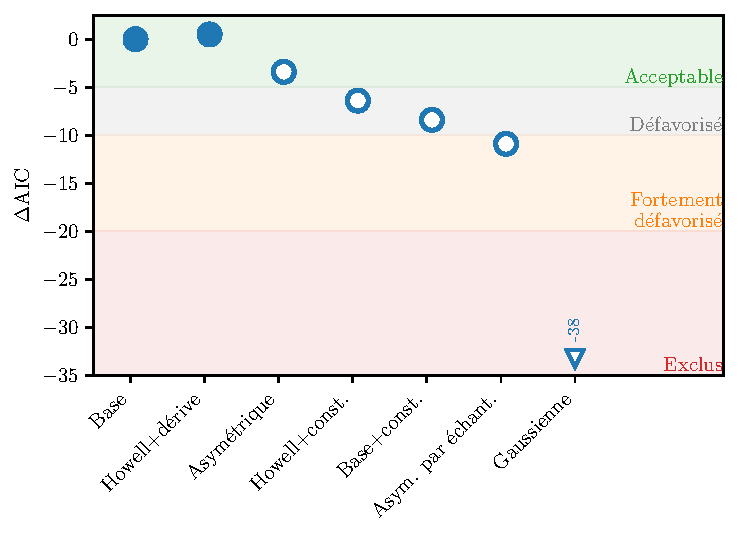
\includegraphics[width=.55\linewidth]{mod_comp_zonly-fr.pdf}
    \caption[$\Delta$AIC entre le modèle de base et les autres modèles sans
    utiliser le LsSFR]{$\Delta$AIC entre le modèle de référence et les autres
        modèles sans utiliser le LsSFR (voir Tableau~\ref{tab:comp_zonly}). La
        légende est la même qu'en Figure~\ref{fig:mod_comp}. En revanche, la
        robustesse des résultats concernant l'inaptitude des modèles
        non-dérivants à représenter correctement les données diminue, même si
        les meilleurs modèles sont toujours ceux incluant une dérive (marqueurs
    pleins).}\label{fig:mod_comp_zonly}
\end{SCfigure}

Nous rapportons également qu'une implémentation de ces travaux avec des coupes
dites «~superconservatives~», avec $z_{\rm lim, SDSS} = 0,10$, $z_{\rm lim, PS1}
= 0,20$, $z_{\rm lim, SNLS} = 0,30$ pour un total de 244 SNe~Ia a également été
effectuée. Ces coupes discriminent alors d'autant plus les modèles
non-dérivants, tous leurs AIC chutant plus que le modèle Howell+dérive~;
notamment le modèle asymétrique passe sous la barre des $\Delta$AIC < -20. La
Figure~\ref{fig:mod_comp_sc} représente ces résultats. Un ultime test a été de
considérer 200 échantillons de la taille de notre échantillon conservatif, mais
tirés aléatoirement de l'échantillon fiduciel. Pour les modèles non-dérivants,
nous trouvons alors une répartition des $\Delta$AIC autour de la valeur fiducielle,
mais rarement meilleure que l'échantillon conservatif initial. Pour le modèle
Howell+dérive nous trouvons la même répartition, mais jamais meilleure que le
modèle de base, qui reste donc encore dans cette étude le modèle de référence,
voir Figure~\ref{fig:mod_comp_cal}.

% \begin{figure}[ht]
% %    \centering
%     \begin{subfigure}[]{.45\linewidth}
% %        \centering
%         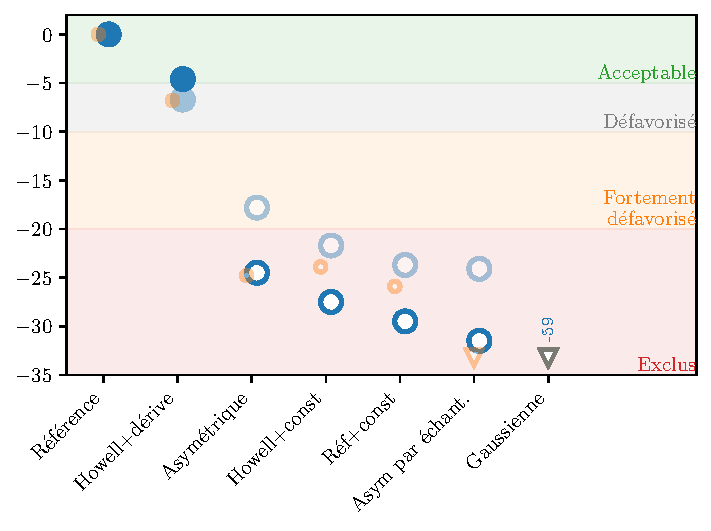
\includegraphics[width=\linewidth]{mod_comp-supercut}
% %        %\captionsetup{justification=centering}
%         \caption[$\Delta$AIC pour un échantillon superconservatif de 244
%         SNe~Ia]{$\Delta$AIC entre le modèle de base et les autres modèles, avec
%             cette-fois ci en petits marqueurs oranges les résultats de l'étude
%             pour un échantillon «~superconservatif~» constitué de 244 SNe~Ia. Le
%             modèle Howell+dérive n'est pas fortement défavorisé par cette coupe,
%             alors que les modèles non-dérivants y sont plus sensibles, tous
%         voyant leur valeur d'AIC baisser significativement.}
%         \label{fig:mod_comp_sc}
%     \end{subfigure}
%     \hfill
%     \begin{subfigure}[]{.45\linewidth}
% %        \centering
%         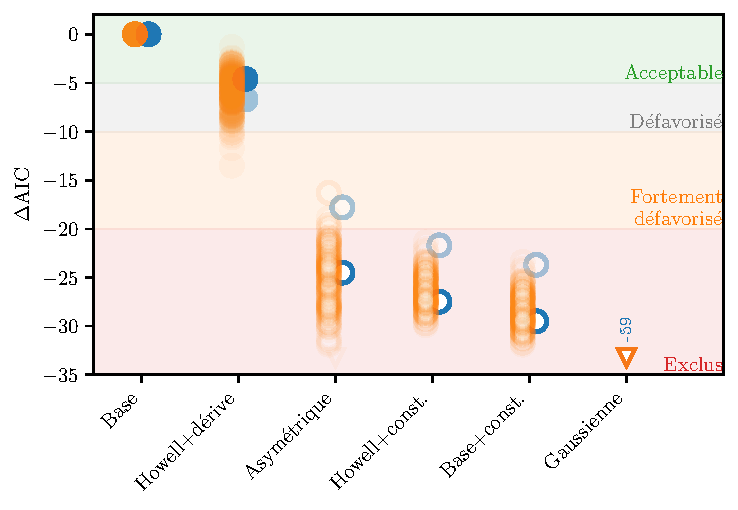
\includegraphics[width=\linewidth]{mod_comp_6mod}
% %        %\captionsetup{justification=centering}
%         \caption[$\Delta$AIC pour des échantillons de taille conservative tirés
%         aléatoirement de l'échantillon fiduciel]{$\Delta$AIC entre le modèle de
%             base et les autres modèles, avec ici en marqueurs orange les
%             résultats pour 200 modèles ajustés avec des données de la taille de
%             l'échantillon conservatif mais tirées aléatoirement de l'échantillon
%             fiduciel. Bien qu'une augmentation du $\Delta$AIC par rapport au cas
%             fiduciel survient par moment, aucun modèle n'obtient de meilleur AIC
%             que le modèle de base, s'imposant encore comme le modèle de
%         référence.}
%         \label{fig:mod_comp_cal}
%     \end{subfigure}
%     \caption{Tests finaux de l'étude de l'évolution de l'étirement avec le
%     redshift.}
% \end{figure}

\begin{SCfigure}[0.8][ht!]
    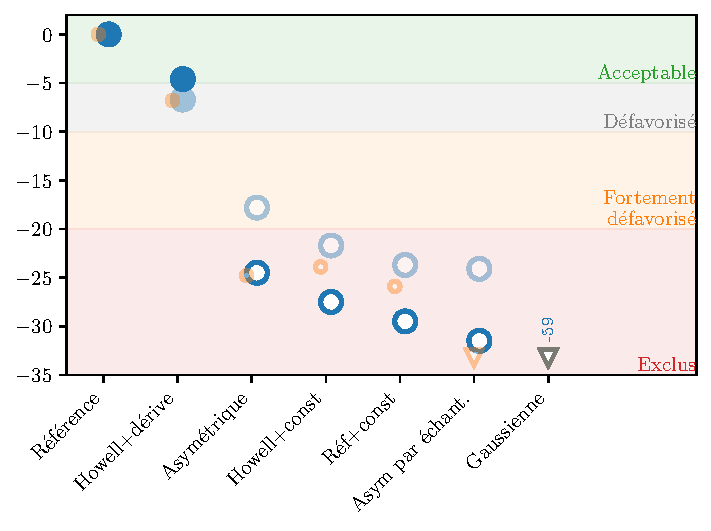
\includegraphics[width=.55\linewidth]{mod_comp-supercut}
    \caption[$\Delta$AIC pour un échantillon superconservatif de 244
    SNe~Ia]{$\Delta$AIC entre le modèle de base et les autres modèles, avec
        cette-fois ci en petits marqueurs oranges les résultats de l'étude
        pour un échantillon «~superconservatif~» constitué de 244 SNe~Ia. Le
        modèle Howell+dérive n'est pas fortement défavorisé par cette coupe,
        alors que les modèles non-dérivants y sont plus sensibles, tous
    voyant leur valeur d'AIC baisser significativement.}
    \label{fig:mod_comp_sc}
\end{SCfigure}

\begin{SCfigure}[0.8][ht!]
    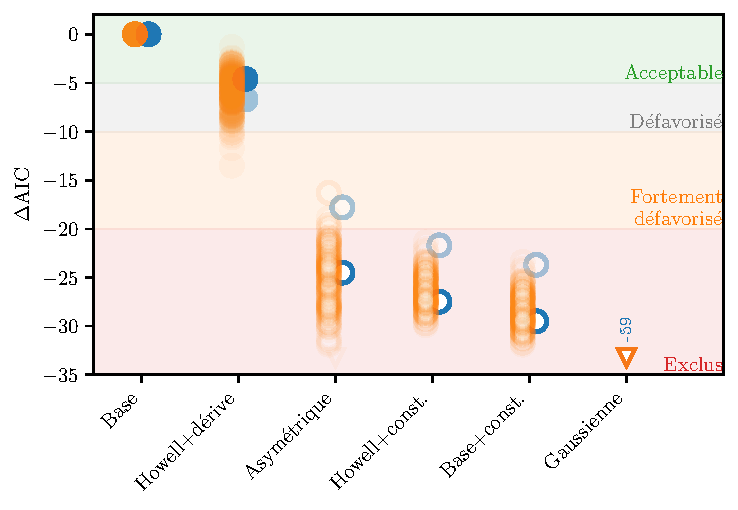
\includegraphics[width=.55\linewidth]{mod_comp_6mod}
    \caption[$\Delta$AIC pour des échantillons de taille conservative tirés
    aléatoirement de l'échantillon fiduciel]{$\Delta$AIC entre le modèle de
        base et les autres modèles, avec ici en marqueurs orange les
        résultats pour 200 modèles ajustés avec des données de la taille de
        l'échantillon conservatif, mais tirées aléatoirement de l'échantillon
        fiduciel. Bien qu'une augmentation du $\Delta$AIC par rapport au cas
        fiduciel survienne par moment, aucun modèle n'obtient de meilleur AIC
        que le modèle de base, celui-ci s'imposant encore comme le modèle de
    référence.}
    \label{fig:mod_comp_cal}
\end{SCfigure}

\subsection{Discussion}\label{ssec:disc}

À notre connaissance, la modélisation de la dérive des redshifts des SNe~Ia n'a
jamais été explicitement utilisée dans les analyses cosmologiques, bien qu'un
formalisme de hiérarchie bayésienne tel que UNITY \citep{rubin2015}, BAHAMAS
\citep{shariff2016} ou Steve \citep{hinton2019} puisse facilement le permettre
\citep[voir, par exemple, les sections 1.3 et 2.5 de][]{rubin2015}. Ne pas le
faire constitue un problème de second ordre pour la cosmologie avec les SNe~Ia
car cela n'affecte que la manière dont le biais de \textsc{Malmquist} est pris
en compte. Tant que le paramètre de normalisation $\alpha$ de la relation de
\textsc{Phillips} \citep{phillips1993} ne dépend pas du redshift \citep[une
étude qui dépasse le cadre de cette thèse, mais voir, par
exemple][]{scolnic2018}, les magnitudes corrigées de l'étirement utilisées pour
la cosmologie sont effectivement insensibles à la distribution d'étirement
sous-jacente pour les échantillons complets. Cependant, les enquêtes présentent
généralement un biais de \textsc{Malmquist} significatif pour la moitié
supérieure de leur distribution de redshift de SNe. Par conséquent, une mauvaise
modélisation de la distribution d'étirement sous-jacente biaisera les magnitudes
dérivées des SNe de ces études.

Les techniques de correction du biais de \textsc{Malmquist} couramment
utilisées, telles que le formalisme BBC, supposent des fonctions Gaussiennes
asymétriques par échantillon pour modéliser les distributions d'étirement et de
couleur sous-jacentes. Comme le montre la Section~\ref{sec:xres} cependant, une
telle distribution par échantillon est exclue par rapport à notre modèle de
dérive. Contrairement à ce que \citep[Section 2]{scolnic2016} et \citep[Section
5.4]{scolnic2018} ont suggéré, à savoir que les études traditionnelles couvrent
des plages de redshift suffisamment limitées pour que l'approche par échantillon
tienne compte des dérives implicites du redshift, une modélisation directe de la
dérive avec le redshift est donc plus appropriée qu'une approche par
échantillon. Nous ajoutons ici qu'au fur et à mesure que les relevés
cosmologiques modernes tentent de couvrir des plages de redshift de plus en plus
larges afin de réduire les incertitudes systématiques de calibration, cette
approche par échantillon devient moins valide, notamment pour PS1, le
\textit{Dark Energy Survey} \citep[DES,][]{abbott2019}, et, bientôt, le LSST
\citep{ivezic2019}.

Nous illustrons Figure~\ref{fig:bbc_pdf_ps1} la différence de prédiction de la
distribution de l'étirement sous-jacent entre la modélisation asymétrique par
échantillon et notre modèle de dérive de référence pour l'échantillon PS1. Notre
modèle est bimodal, et l'amplitude relative de chaque mode dépend de la fraction
de jeunes et vieilles SNe~Ia dans l'échantillon en fonction du redshift~: plus
la fraction de vieilles SNe~Ia est élevée (à un faible redshift), plus
l'amplitude du mode d'étirement faible spécifique aux vieilles SNe~Ia est élevé.
Cette dépendance avec le redshift des distributions d'étirement sous-jacentes
est représentée par des couleurs allant du bleu au rouge sur la
Figure~\ref{fig:bbc_pdf_ps1} pour la gamme de redshift couvert par l'ensemble de
PS1. L'histogramme des $x_1$ observés suit le modèle que nous avons défini en
utilisant la somme des distributions sous-jacentes individuelles au redshift de
chaque SN du sondage (en noir). Comme prévu, les deux approches de modélisation
diffèrent surtout dans la partie négative de la distribution des étirements de
SNe. La distribution Gaussienne asymétrique passe par le milieu de la
distribution bimodale, surestimant le nombre de SNe~Ia à $x_1 \approx 0,7$ et
le sous-estimant à $x_1 \approx 1,7$ par rapport à notre modèle de dérive de
référence pour les redshifts typiques des SNe de PS1. Cela signifie que la
magnitude standardisée corrigée du biais d'une SN estimée à un redshift affecté
par la sélection observationnelle serait biaisée par une mauvaise modélisation
de la véritable distribution d'étirement sous-jacente.

\begin{figure}[ht]
    \centering
    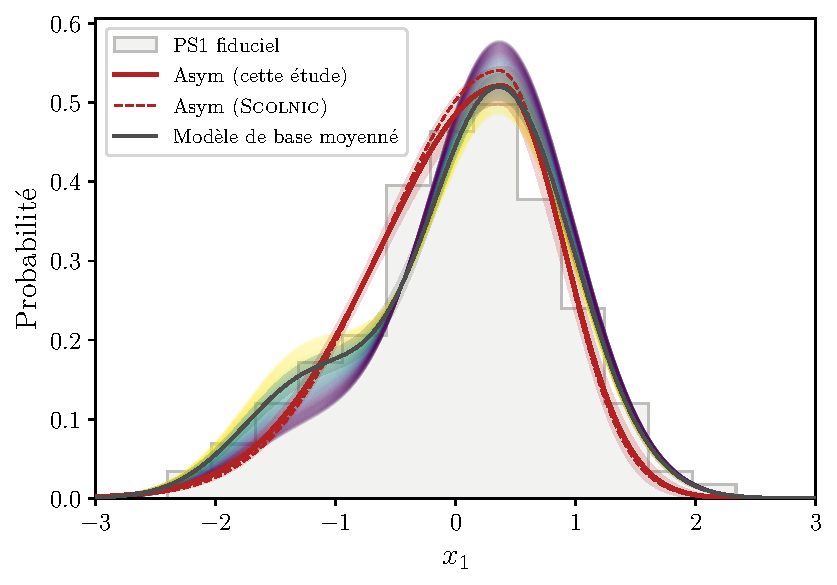
\includegraphics[width=.75\linewidth]{bbc_comp_PS1_hist-nr_viridis.pdf}

    \caption[Comparaison des modélisations de BBC et de notre modèle de
    référence sur l'histogramme des étirements de PS1]{Distribution de
        l'étirement des SNe~Ia de PS1 issus d'un ajustement \texttt{SALT2.4}
        ($x_1$) pour toutes les données du sondage, au-delà de notre limite
        fiducielle de redshift (histogramme gris). Cette distribution est
        supposée être un tirage aléatoire de la distribution d'étirement
        sous-jacente. Les lignes rouges montrent le modèle BBC de cette
        distribution sous-jacente (Gaussienne asymétrique). La ligne pleine (et
        sa bande) est notre meilleur ajustement (et son erreur)~; la ligne
        pointillée montre le résultat de~\cite{scolnic2018}. La ligne noire (et
        sa bande) montre notre modélisation de référence la mieux ajustée (et
        son erreur, voir Tableau~\ref{tab:modelresults}) qui inclut la dérive du
        redshift. À titre d'illustration, nous montrons (coloré du jaune au
        violet avec des redshifts croissants) l'évolution de la distribution
        d'étirement sous-jacente en fonction du redshift pour la plage de
    redshift couverte par toutes les données de PS1.}
    \label{fig:bbc_pdf_ps1}

\end{figure}

L'évaluation de l'amplitude de ce biais de magnitude pour la cosmologie fait
l'objet du Chapitre~\ref{ch:snana}, en utilisant notre modèle de référence
(Équation~\ref{eq:stretchz}) à la place du modèle par échantillon. Cependant,
nous avons déjà mis en évidence que même si un modèle par échantillon sans
dérive pouvait donner des résultats comparables dans la partie limitée en volume
des différents échantillons, ces modèles seraient différents lorsqu'ils
seraient extrapolés à des redshifts plus élevés, précisément là où la
distribution sous-jacente sera importante pour corriger les biais de
\textsc{Malmquist}.

À l'ère de la cosmologie moderne, où nous visons à mesurer $w_0$ à un niveau
inférieur au pourcentage et $w_a$ avec une précision de 10\% \citep[par
exemple,][]{ivezic2019}, nous soulignons que la modélisation correcte de la
dérive potentielle avec le redshift des SNe~Ia doit être étudiée plus
profondément et qu'il faut faire attention lorsque nous utilisons des
échantillons qui sont affectés par des effets de sélection observationnels.

\section{Conclusion}\label{ssec:xccl}

Nous avons présenté une première étude de la dérive de la distribution
d'étirement sous-jacente des SNe~Ia en fonction du redshift. Nous avons
construit Chapitre~\ref{ch:sample} des sous-échantillons de SNe effectivement
limités en volume à partir de l'ensemble de données Pantheon \citep[][SDSS, PS1,
SNLS]{scolnic2018} auxquels nous avons ajouté les données HST et SNfactory
\citep{rigault2020} pour les intervalles à haut et bas redshifts,
respectivement. Nous n'avons considéré que les SNe qui ont été découvertes dans
la plage de redshifts de chaque enquête dans laquelle les effets de sélection
observationnels sont négligeables, de sorte que les étendues de SNe~Ia observées
constituent un échantillon aléatoire de la véritable distribution sous-jacente.
Nous avons ainsi obtenu un échantillon fiduciel de base de 569 SNe~Ia (422 SNe
lorsque des coupes plus conservatives sont appliquées). 

Suivant les prédictions de~\cite{rigault2020}, nous avons introduit un modèle de
dérive avec le redshift qui dépend de la fraction attendue de SNe~Ia
jeunes et vieilles en fonction du redshift, chaque population d'âge ayant sa
propre distribution d'étirement sous-jacente.

En plus de ce modèle de base, nous avons étudié diverses distributions, y
compris des modèles indépendants du redshift. Nous avons également étudié la
prédiction à partir d'une distribution d'étirement gaussienne asymétrique par
échantillon, utilisée par exemple par l'algorithme de correction de biais de
\textsc{Malmquist} BBC \citep{scolnic2016, kessler2017}. Nos conclusions sont
énumérées ci-dessous.

\begin{enumerate}
    \item La distribution sous-jacente de l'étirement des SNe~Ia est
        significativement dépendante du redshift, comme l'ont suggéré
        précédemment~\cite{howell2007} par exemple, d'une manière que les effets
        de sélection observationnels seuls ne peuvent expliquer. Ce résultat est
        largement indépendant des détails de chaque modèle âge-population~;
    \item Les modèles indépendants du redshift sont quantitativement exclus
        comme descriptions appropriées des données par rapport à notre modèle de
        base, d'autant plus que la statistique de l'échantillon augmente. Ce
        modèle suppose que (1) la population plus jeune a une distribution
        d'étirement gaussienne unimodale tandis que la distribution d'étirement
        de la population plus âgée est bimodale, l'un des modes étant le même
        que celui de la population jeune, et (2) que l'évolution de la fraction
        relative des SNe~Ia jeunes et vieilles suit la prédiction
        de~\cite{rigault2020}. Ce second résultat soutient l'existence de
        populations de SNe~Ia jeunes et vieilles, en accord avec les études de
        taux de production de SNe \citep{mannucci2005, scannapieco2005,
        sullivan2006, aubourg2008}.
    \item Les modèles utilisant des distributions Gaussiennes asymétriques
        basées par échantillon, comme par exemple ceux utilisés dans
        l'implémentation actuelle de BBC, sont exclus comme étant de bonnes
        descriptions des données par rapport à notre modèle de dérive. Cela
        signifie que l'approche basée par échantillon ne tient pas compte avec
        précision de la dérive du redshift, un problème qui sera exacerbé par
        des sondages couvrant des plages de redshifts de plus en plus grandes.
        Par conséquent, même si les degrés de liberté supplémentaires
        nécessaires peuvent être acceptables étant donné le grand nombre de
        SNe~Ia dans les études cosmologiques, l'extrapolation des distributions
        des propriétés des SNe~Ia de la partie limitée en volume d'une
        étude à sa partie limitée en magnitude et affectée par le biais de
        \textsc{Malmquist} serait toujours inexacte en raison de l'évolution
        avec le redshift.
    \item Compte tenu de l'ensemble de données actuel, nous suggérons
        l'utilisation du modèle de population d'étirements évoluant avec le
        redshift suivant~:
        \begin{align*}\label{eqconclusion:stretchz}
            X_1\left(z \right) =
            \delta(z)&\times\mathcal{N}(\mu_1,\sigma_1{}^2)\,+\nonumber\\
            (1-\delta(z))&\times \left[a\times\mathcal{N}(\mu_1,\sigma_1{}^2) +
            (1-a)\times\mathcal{N}(\mu_2,\sigma_2{}^2)\right],
            \tag{\ref{eq:stretchz}}
        \end{align*}
        avec $a=0.51$, $\mu_1=0.37$, $\mu_2=-1.22$, $\sigma_1=0.61$, et
        $\sigma_2=0.56$ (voir Tableau~\ref{tab:modelresults}), et d'utiliser
        le modèle de dérive de la population d'âge avec le redshift suivant~:
        \begin{align*}
            \delta(z) & = \left( K^{-1} \times (1+z)^{-2.8} +1 \right)^{-1}
            \tag{\ref{eq:deltaz}}
        \end{align*}
        avec $K=0.87$.
\end{enumerate}

La prochaine étape de cette ligne d'analyse consiste à incorporer notre modèle
dans le cadre de \snana\ \citep{kessler2009a}, un ensemble de logiciels de
production de données simulées basées sur les données réelles d'observation.
Cela va permettre à la fois de tenir compte plus précisément des fonctions de
sélection observationnelles et de tester l'effet de notre modèle sur la
détermination des paramètres cosmologiques. Cette étude fait l'objet du chapitre
suivant.

% \bibliographystyle{../main/aa_url}
% \shorthandoff{:}
% \bibliography{../chapters/99_references}

\end{document}
